\chapter{Analysis}

\section {Actors}
\begin{itemize}
    \item \textbf{Unregistered User}: A visitor who has not logged in on the platform.
    \item \textbf{Registered User}: A user who has created an account on the platform. 
    \item \textbf{Manager}: A registered user with administrative privileges. 
\end{itemize}

\section{Requirements}
\textbf{Unregistered User}:

\begin{itemize}
    \item Register/Login:
    \begin{itemize}
        \item Create a new account to access additional features.
        \item Use valid credentials (email and password) to log into the account.
    \end{itemize}
    \item Browse Media Contents.
    \item Search and Filter Media Contents:
    \begin{itemize}
        \item Find specific manga or anime by title.
        \item Utilize basic filtering options to refine the media content list.
    \end{itemize}
    \item View Media Content Trends.
    \item View Media Content:
    \begin{itemize}
        \item View limited information about each media content.
    \end{itemize} 
    \item View Media Content Details:
    \begin{itemize}
        \item View detailed information about each media content.
        \item View reviews and ratings for each media content.
        \item View number of likes for each media content.
    \end{itemize}
    \item Browse Users.
    \item Search Users by Username.
    \item View User:
    \begin{itemize}
        \item View limited information about each user.
    \end{itemize} 
    \item View User Details:
    \begin{itemize}
        \item View detailed information about each user.
        \item View anime and manga liked by the user.
        \item View followers and following of the user.
    \end{itemize}
\end{itemize}

\textbf{Registered User}:

\begin{itemize}
    \item Logout.
    \item Browse Media Contents.
    \item Search and Filter Media Contents:
    \begin{itemize}
        \item Find specific manga or anime by title.
        \item Utilize basic filtering options to refine the media content list.
    \end{itemize}
    \item View Media Content Trends.
    \item View Media Content:
    \begin{itemize}
        \item View limited information about each media content.
    \end{itemize} 
    \item View Media Content Details:
    \begin{itemize}
        \item View detailed information about each media content.
        \item View reviews and ratings for each media content.
        \item View number of likes for each media content.
    \end{itemize}
    \item Browse Users.
    \item Search Users by Username.
    \item View User:
    \begin{itemize}
        \item View limited information about each user.
    \end{itemize} 
    \item View User Details:
    \begin{itemize}
        \item View detailed information about each user.
        \item View anime and manga liked by the user.
        \item View followers and following of the user.
    \end{itemize}
    \item Profile Management:
    \begin{itemize}
        \item Edit and update personal information (e.g., profile picture, bio).
        \item Delete own profile.
    \end{itemize}
    \item Like/Unlike Media Contents.
    \item Follow/Unfollow Users.
    \item Review Media Contents:
    \begin{itemize}
        \item Add comment and rating to manga and anime.
        \item Edit/Delete own reviews.
    \end{itemize}
    \item Advanced Recommendations:
    \begin{itemize}
        \item Receive media content suggestions based on user interactions and personal information.
        \item Receive users suggestions based on user interactions.
    \end{itemize}
\end{itemize}

\textbf{Manager}(Registered User with Administrative Features):

\begin{itemize}
    \item Logout.
    \item Browse Media Contents.
    \item Search and Filter Media Contents:
    \begin{itemize}
        \item Find specific manga or anime by title.
        \item Utilize basic filtering options to refine the media content list.
    \end{itemize}
    \item View Media Content Trends.
    \item View Media Content:
    \begin{itemize}
        \item View limited information about each media content.
    \end{itemize} 
    \item View Media Content Details:
    \begin{itemize}
        \item View detailed information about each media content.
        \item View reviews and ratings for each media content.
        \item View number of likes for each media content.
    \end{itemize}
    \item Browse Users.
    \item Search Users by Username.
    \item View User:
    \begin{itemize}
        \item View limited information about each user.
    \end{itemize} 
    \item View User Details:
    \begin{itemize}
        \item View detailed information about each user.
        \item View anime and manga liked by the user.
        \item View followers and following of the user.
    \end{itemize}
    \item Analytics Dashboard:
    \begin{itemize}
        \item View user analytics (distribution and app rating).
        \item View manga analytics (trends and average rating).
        \item View anime analytics (trends and average rating).
    \end{itemize}
   
    \item Content Management:
    \begin{itemize}
        \item Add new media content (manga and anime).
        \item Update/Remove existing media content.
    \end{itemize}
\end{itemize}

\section{Non Functional Requirements}

\textbf{Performance}

\begin{itemize}
    \item Response Time: The system should have low latency, with pages loading within an acceptable timeframe.
    \item Scalability: The system should be able to handle an increasing number of users and data without significant degradation in performance.
    \item Concurrency: The application should support multiple users simultaneously without performance bottlenecks. For very high traffic scenarios, acceptable delays may be introduced.
    \item Availability: The system should be available 24/7, with minimal downtime for maintenance.
    \item Replication: The system should have data replication to ensure data availability and fault tolerance.
\end{itemize}

\textbf{Security}
\begin{itemize}
    \item Controlled User Operations: Users should only be able to perform operations that they are authorized to do.
\end{itemize}

\textbf{Data Integrity}

\begin{itemize}
    \item Data Consistency: The system should maintain data consistency across all components and databases.
\end{itemize}

\textbf{User Interface}
\begin{itemize}
    \item Responsiveness: The user interface should be responsive, providing a consistent and seamless experience across various devices and screen sizes.
    \item Intuitiveness: The interface should be user-friendly, with clear navigation and easily understandable features.
\end{itemize}

\newpage

\section{UML use case diagram}
\begin{figure}[h]
    \centering
    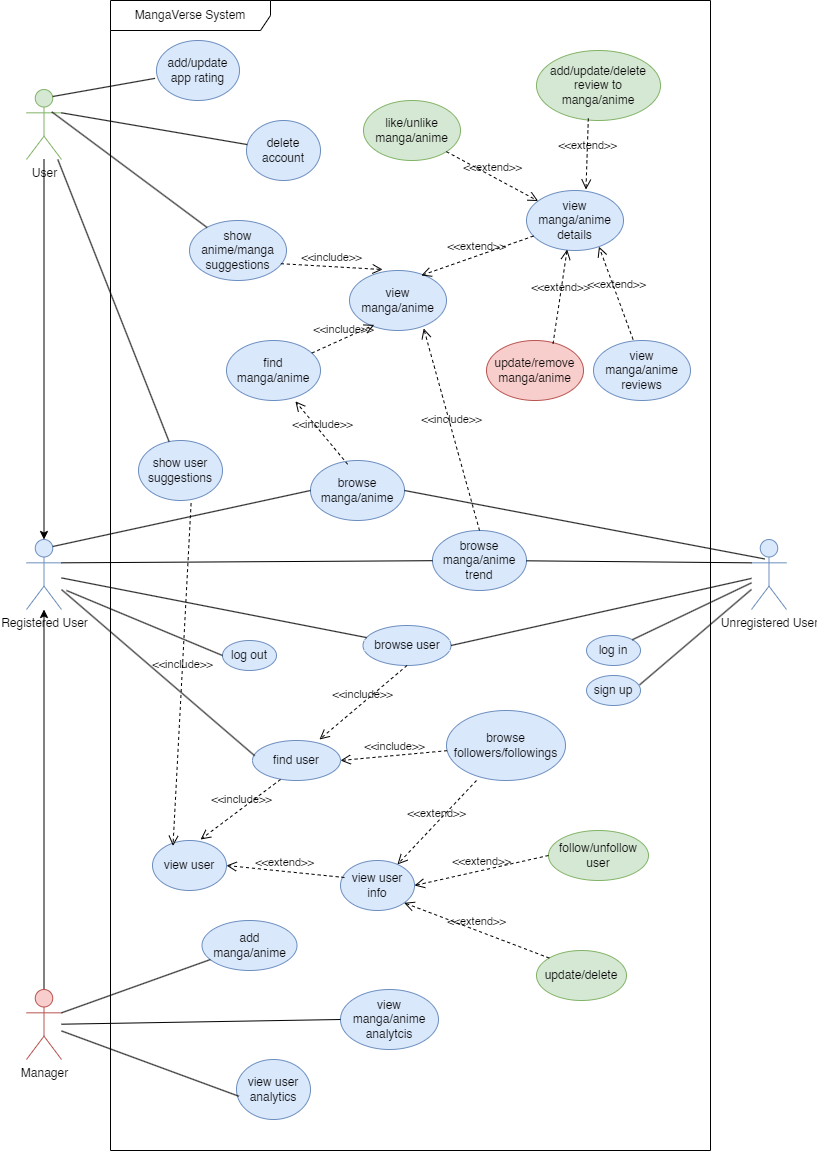
\includegraphics[width=0.82\textwidth]{Media/useCase.png}
    \caption{UML Use Case Diagram}
    \label{uml use case diagram}
\end{figure}

\newpage

\section{UML class diagram}
\begin{figure}[h]
    \centering
    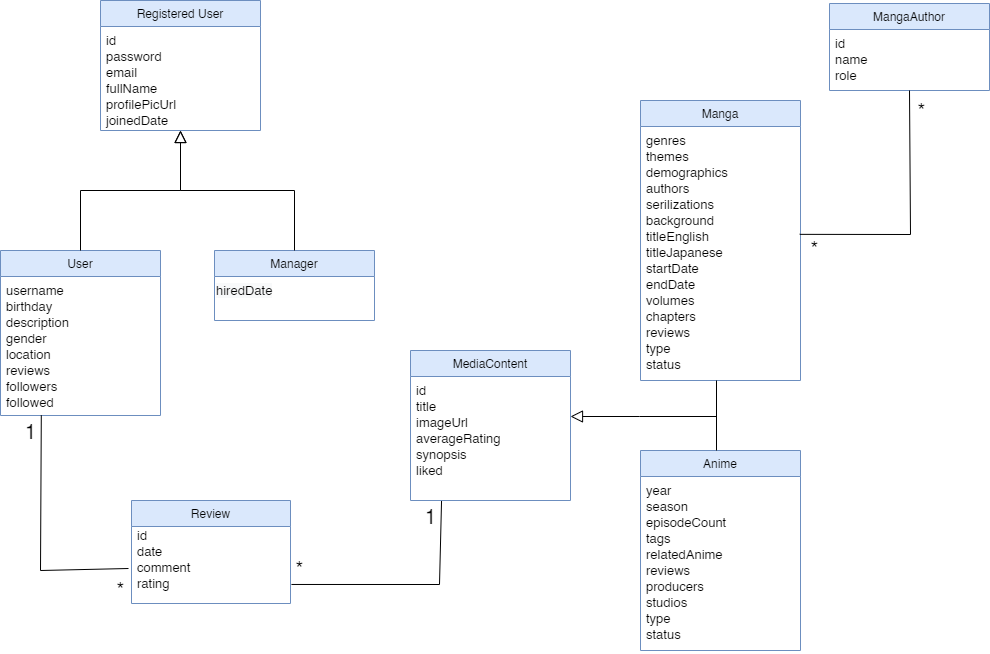
\includegraphics[width=\linewidth]{Media/Class Diagram.png}
    \caption{UML Class Diagram}
    \label{uml class diagram}
\end{figure}

\newpage


\section{Data Modeling}
\subsection{Data Collection}
\textit{Sources:} https://www.kaggle.com/datasets/dbdmobile/myanimelist-dataset?select=users-score-2023.csv, MyAnimeList.net,	anilist.com,  kitsu.io,			  livechart.me,
anime-planet.com,		nofity.moe,	   anisearch.com,		  anidb.net 	

\textit{Description:} Manga, users and scores datasets were collected from MyAnimeList.net site using the official API and another unofficial API (Jikan). The anime datasets were collected from all the sources. 

\textit{Variety:} The datasets contain a variety of data types, including text, numbers, and dates. Anime are collected from 8 different sources. All the information is collected in 4 different csv files.

\textit{Volume:} The datasets contain a large volume of data, with thousands of entries for anime, manga, users, and scores. The total size of the datasets is around 3 GB.

\subsection{Data Cleaning and Preprocessing}
Python scripts were used to clean and preprocess the data. The following steps were performed:
reviews were created by merging the users and scores datasets, and creating comments about the media contents;
the anime dataset was created by putting togethere the diffrerent sources;
the manga dataset was created from MyAnimeList.net;
the users dataset was cleaned and missing information, like email and password, was added.

%add more details about the data cleaning and preprocessing steps